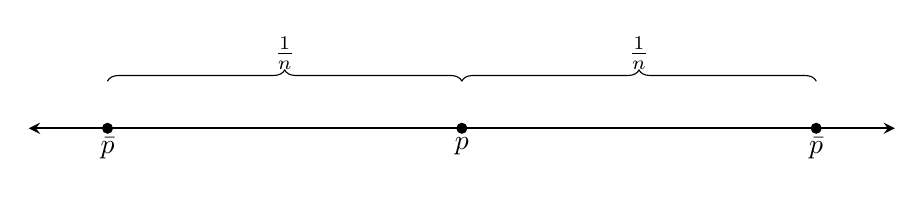
\begin{tikzpicture}[>=stealth, line cap=round]
\def\xL{-4.5}
\def\xC{0}
\def\xR{4.5}
\draw[thick, <->] (-5.5,0) -- (5.5,0);
\fill (\xL,0) circle (2pt);
\fill (\xC,0) circle (2pt);
\fill (\xR,0) circle (2pt);
\node[below] at (\xL,0) {$\bar p$};
\node[below] at (\xC,0) {$p$};
\node[below] at (\xR,0) {$\bar p$};
\draw[decorate, decoration={brace, amplitude=4pt}]
  (\xL,0.6) -- (\xC,0.6)
  node[midway, yshift=10pt] {$\frac{1}{n}$};
\draw[decorate, decoration={brace, amplitude=4pt}]
  (\xC,0.6) -- (\xR,0.6)
  node[midway, yshift=10pt] {$\frac{1}{n}$};
\end{tikzpicture}